\chapter{Marshaling between C\# and C Part 1}
For this chapter, you'll need to create a ChapterFive directory and initialize a Dotnet Console project and to reference ''AdvancedDLSupport'' from nuget.

\section{Struct Layout}
The Layout in Struct is by default set to Sequential and you cannot use Auto layout for marshaling between Managed and Unmanaged code. Explicit Layout allows the you to explicitly define the field offsets in struct layout. This is also what enables you to  create a union in struct.

\lstinputlisting[style=customcs]{codes/Chap5/Chap5Snippet1.cs}

You may have noticed that the Val1 occupied 2 byte slots in the struct rather than Val2 being placed immediately after Val1. This is due to data alignment.  More information on that can be found here: https://software.intel.com/en-us/articles/data-alignment-when-migrating-to-64-bit-intel-architecture

To quote from that link:

\begin{coloredbox}
	The fundamental rule of data alignment is that the safest (and most widely supported) approach relies on what Intel terms "the natural boundaries." Those are the ones that occur when you round up the size of a data item to the next largest size of two, four, eight or 16 bytes. For example, a 10-byte float should be aligned on a 16-byte address, whereas 64-bit integers should be aligned to an eight-byte address. Because this is a 64-bit architecture, pointer sizes are all eight bytes wide, and so they too should align on eight-byte boundaries. - Intel 2018
\end{coloredbox}

The size of the struct shown above is 12 bytes rather than 8 bytes, because the sequential layout rule was being followed. However if you wish to override the behavior on data alignment, you can use Explicit Layout as shown below:
\newpage
\lstinputlisting[style=customcs]{codes/Chap5/Chap5Snippet2.cs}

In this struct, the size would become 8 bytes, because there is no padding required for any dangling member to fits in alignment, so everything fits neatly inside the 8 bytes boundary. Also, in explicit layout, the arrangement of members in struct does not affect how memory is laid out, you define the offsets yourself, so you essentially can arrange the members however you like, though it's recommended to keep member arrangement sequential for readability.

\subsection{Union}
Due to the nature of explicit layout, we can overlap where the field are located in memory by using FieldOffset. If you have for an example have the following code:

\lstinputlisting[style=customcs]{codes/Chap5/Chap5Snippet3.cs}

The size of struct would remain at 1 byte, so no padding is added and both fields are storing into the same memory in the struct.

It is however recommended that you create separate structs for each union definition that you may come across in C native library binding as demonstrated:

\lstinputlisting[style=customcs]{codes/Chap5/Chap5Snippet4.cs}

The resulting size of this struct would be 8 bytes, because it still follows the padding rule for sequential in MyStruct by padding the union struct to fits in the memory boundary.

\subsection{Packing and Size Options for Struct Layout}
You can specify the packing option to respect byte boundary from a multiple of 1 byte to 8 bytes (.Net Core 3.0 and later will support 16 to 32 bytes boundary.)

Size will only be respected if the specified size is bigger than actual size of struct (including padding) however a different behavior results between Mono and CoreCLR when Size is specified to be smaller than actual size of struct. Read Subsection CoreCLR vs Mono that covers this part.

Here an example to demonstrate the differences of each struct with specified Packing and Size.

\lstinputlisting[style=customcs]{codes/Chap5/Chap5Snippet5.cs}
\newpage
And the output for each struct is as followed:
\newline \newline
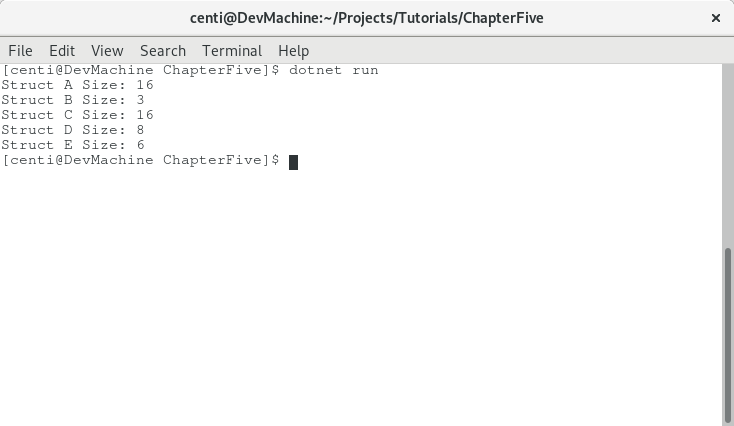
\includegraphics[width=\textwidth]{ChapFiveConsole}

\begin{enumerate}
	\item Struct A have Size specified and is larger than the actual size of struct with padding (which is 1 byte size for Struct A actual size.)
	\item Struct B have size specified to 1 byte size struct with packing alignment of 8 bytes boundary. There are 2 separate behavior that results from this, in CoreCLR, the struct would result as 3 bytes size struct while Mono results in 4 bytes size.
	\item Struct C size is 16 bytes even though it's actual size is 9 bytes, this is how padding affects the size of the struct. If padding is set to 1, we would see the Struct C size become 9 bytes long.
	\item Struct D size is 8 bytes as described above, the actual size of struct is 5 bytes long and because of the specified padding, it is padded to 8 bytes boundary.
	\item Struct E size is 6 bytes as opposed to Struct D, because packing is specified to pad struct to the multiple of 2 bytes.
\end{enumerate}

\subsection{Technical Note on Packing}
While Natural Boundaries are something to keep in mind for 64 bit data alignment, it is done differently for 32 bit architecture, it's packed in the multiple of 4 bytes. And in CoreCLR prior to 3.0, 8 bytes packing is the most that can be used and .Net Core 3.0 and later will have packing supporting 16 and 32 bytes boundary to support Vector128<T> and Vector256<T>. 

\subsection{What is the Difference between sizeof and Marshal.SizeOf}
Marshal.SizeOf tells you how much bytes are needed to allocate the structure in unmanaged environment and sizeof tells you how much memory required to allocate the structure in managed environment. The SizeOf keyword cannot accept managed object member in the struct such as reference type like string due to language limitation (but not technical limitation of CLR), but Unsafe.SizeOf can and it utilize the underlying CIL sizeof opcode.

Let's assume we have the following code to demonstrate the difference:

\lstinputlisting[style=customcs]{codes/Chap5/Chap5Snippet6.cs}

And the output of that program will be:
\newline
\newline
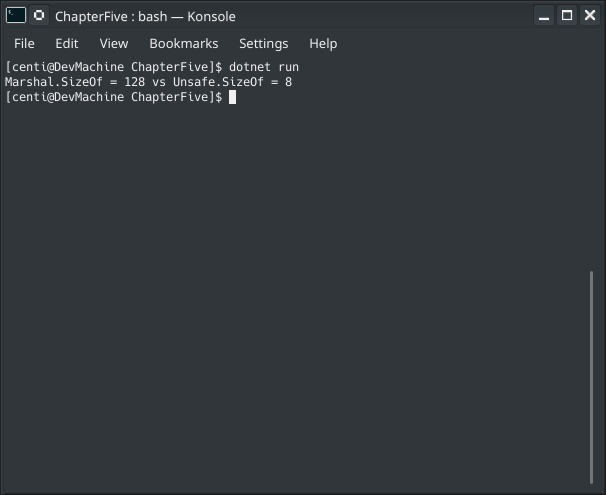
\includegraphics[width=\textwidth]{ChapFiveConsoleTwo}
\newpage

In a managed environment, the string would be a reference type and on 64 bit architecture, the pointer would be 8 bytes long, 4 bytes long on a 32 bit architecture. However, because we explicitly define that our string in a struct is a By Value String, it is essentially a fixed length array of characters of specific encoding (in this case, Ansi Encoding.) The size of struct \textit{should} be 128 bytes long for marshaling purpose.

\subsection{CoreCLR vs Mono Struct Alignment}
In CoreCLR, the struct size is emphasized on the packing, not on alignment, but on Mono, it's emphasized on alignment along with packing. So a struct defined as thus:

\lstinputlisting[style=customcs]{codes/Chap5/Chap5Snippet10.cs}

Have Marshal.SizeOf result of 3 on CoreCLR while it's 4 on Mono, Mono rounded it up to Natural Alignment Boundary.

\subsection{Fixed Size Array}
You can allocate a fixed sized array within a struct, but it is restricted to the following types: bool, byte, char, short, int, long, sbyte, ushort, uint, ulong, float, or double. Though there is a proposal for this change to allow user-defined structs to be used for fixed sized array: \newline \newline
https://github.com/dotnet/csharplang/blob/master/proposals/fixed-sized-buffers.md
\newline \newline

The fixed statement require an unsafe modifier for struct and you can create a fixed size array by writing the following:

\lstinputlisting[style=customcs]{codes/Chap5/Chap5Snippet7.cs}

This is a struct that is allocated for 128 bytes with a fixed size array of bytes. There is one thing to note about this, fixed size buffer is \textbf{NOT} bound checked, it is a pointer to the first element of the array in struct hence this is why unsafe modifier is required.

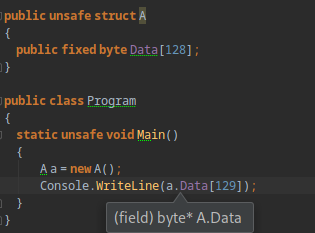
\includegraphics[width=7cm, height=5cm]{ChapFiveMouseOver}
\newpage

\subsection{By Value Array of Struct}
C\# does not have a concept for By Value Array of Struct though there is an upcoming proposal to introduce support for this. At this time, fixed statement is restricted to certain primitive types. There are few possible approach that you can accomplish By Value Array of Structs, one of them is to allocate certain amount of bytes to accommodate the space required to store a number of struct elements with a by value byte array. The following code will demonstrate on how to accomplish this:

\lstinputlisting[style=customcs]{codes/Chap5/Chap5Snippet8.cs}
\newpage
Another approach is a little more elegant approach that apply similar concept as above:

\lstinputlisting[style=customcs]{codes/Chap5/Chap5Snippet9.cs}

This snippet was originally written by Tanner Gooding.
\newline
\newline
The idea with this approach is that you leverage the StructLayout as mentioned in previous section to allocate large enough struct to accommodate the size of By Value Array and you introduce first element field so that field can be used as a reference to read/store other elements. The indexer property simply make the code easier to read, avoiding unneeded casting on external code and to ensure that it is bound checked. This approach is recommended for By Value Array of Struct Marshaling.
